\documentclass[a4paper,12pt]{article}
\usepackage[left=2cm,right=2cm,top=2cm,bottom=2cm]{geometry} % Do ustawień marginesów
\usepackage{multicol} % Dla podziału na kolumny
\usepackage{ragged2e} % Dla justowania tekstu
\usepackage{graphicx} % Required for inserting images
\usepackage{float}
\usepackage{caption}
\usepackage{amsmath} % Math formulas
\usepackage{amssymb} % Symbols
\usepackage[svgnames]{xcolor}
\usepackage[colorlinks=true, urlcolor=blue, linkcolor=black, citecolor=orange]{hyperref} % Hyperlinks
\usepackage{polski} % Polish language
\usepackage[utf8]{inputenc} % Text encoding
\usepackage{enumitem} % Pakiet do elastycznego sterowania listami
\usepackage{indentfirst}
\usepackage{array}
\usepackage{longtable}

\setlist[itemize]{itemsep=0pt, topsep=0pt}

\begin{document}

% Górna część strony
\noindent
\begin{minipage}{0.5\textwidth}
    \raggedright
    \textbf{Piotr Durniat} \\
    I rok, Fizyka \\
    Wtorek, 8:00-10:15 \\
    \vspace{0.5cm}
    \vspace{0.5cm}
\end{minipage}%
\begin{minipage}{0.5\textwidth}
    \raggedleft
    Data wykonania pomiarów: \\
    06.05.2025 \\
    \vspace{0.5cm} % Dodatkowa linia przerwy
    Prowadząca: \\
    dr Iwona Mróz
\end{minipage}

% Tytuł ćwiczenia
\vspace{2cm} % Odstęp
\begin{center}
    \LARGE \textbf{Ćwiczenie nr 30} \\[0.5cm]
    \Large \textbf{Wyznaczanie względnej gęstości cieczy i ciał stałych}
\end{center}

% Reszta treści
\vspace{1cm} % Kolejny odstęp
\noindent

\tableofcontents
\newpage

% ---------- WSTĘP TEORETYCZNY ----------
\section{Wstęp teoretyczny}

\subsection*{Ciężar właściwy ciała}

Ciężar właściwy ciała ($\gamma$) jest to stosunek ciężaru ciała ($P$) do jego objętości ($V$), wyrażony wzorem:

\begin{equation*}
    \gamma = \frac{P}{V}
\end{equation*}


W ogólności ciała rozszerzają się, gdy rośnie temperatura, tym samym ponieważ masa pozostaje stała, to gęstość ciała maleje. Istnieją jednak wyjątki od tej reguły, np. woda, która w temperaturze poniżej 4 stopni Celsjusza zachowuje się anomalnie - wzrasta jej gęstość wraz ze wzrostem temperatury, a poniżej 4 stopni Celsjusza zachowuje się odwrotnie - maleje gęstość wraz ze wzrostem temperatury.

\subsection*{Waga Jolly'ego}

Wyprowadzenie wzoru na względną gęstość ciała stałego wyznaczonego za pomocą wagi Jolly'ego:

Waga Jolly'ego to przyrząd wykorzystujący prawo Hooke'a do pomiaru siły wyporu i wyznaczenia gęstości ciał. Zgodnie z prawem Hooke'a, siła sprężystości jest proporcjonalna do odkształcenia sprężyny i wyraża się wzorem:
\begin{equation*}
    F_s = -k \cdot \Delta x
\end{equation*}
gdzie $k$ jest współczynnikiem sprężystości, a $\Delta x$ oznacza zmianę długości sprężyny.

Rozważmy dwa przypadki pomiarowe. W pierwszym przypadku, gdy ciało znajduje się w powietrzu, zachodzi równowaga sił:
\begin{equation*}
    F_s + F_g = 0
\end{equation*}
gdzie $F_g$ to siła ciężkości działająca na ciało. Po podstawieniu otrzymujemy:
\begin{equation*}
    -k(h_p - h_0) + \rho_{s} V g = 0
\end{equation*}

gdzie $h_p$ to położenie wskazówki wagi z ciężarkiem w powietrzu, a $h_0$ to położenie wskazówki bez obciążenia. Z tego wynika, że:

\begin{equation}
    \label{eq:case1}
    k(h_p - h_0) = \rho_{s} V g
\end{equation}

W drugim przypadku, gdy ciało jest zanurzone w cieczy, równowaga sił uwzględnia dodatkowo siłę wyporu:
\begin{equation*}
    F_s + F_{\text{wypór}} = F_g
\end{equation*}

Po podstawieniu otrzymujemy:

\begin{equation*}
    -k(h_w - h_0) + \rho_{c} V g = \rho_{s} V g
\end{equation*}

gdzie $h_w$ to położenie wskazówki wagi z ciężarkiem zanurzonym w cieczy. Przekształcając to równanie, uzyskujemy:
\begin{equation}
    \label{eq:case2}
    k(h_w - h_0) = (\rho_{s} - \rho_{c}) V g
\end{equation}

Aby wyznaczyć względną gęstość ciała, dzielimy równanie \eqref{eq:case1} przez równanie \eqref{eq:case2}:
\begin{equation*}
    \frac{h_p - h_0}{h_w - h_0} = \frac{\rho_{s}}{(\rho_{s} - \rho_{c})}
\end{equation*}

Następnie przekształcamy to wyrażenie:
\begin{equation*}
    \frac{h_w - h_0}{h_p - h_0} = \frac{\rho_{s} - \rho_{c}}{\rho_{s}}
\end{equation*}

\begin{equation*}
    1 - \frac{h_w - h_0}{h_p - h_0} = \frac{\rho_{c}}{\rho_{s}}
\end{equation*}

Odwracając ostatnie równanie, otrzymujemy wzór na względną gęstość ciała stałego:
\begin{equation}
    \label{eq:wzgledna_gestosc_jolly}
    R = \frac{\rho_{s}}{\rho_c} = \frac{h_p - h_0}{h_p - h_w}
\end{equation}

W powyższym wzorze:
\begin{itemize}
    \item $\rho_{s}$ to gęstość badanego ciała stałego,
    \item $\rho_c$ to gęstość cieczy,
    \item $h_p$ to położenie wskazówki wagi, gdy ciężarek znajduje się w powietrzu (na górnej szalce),
    \item $h_w$ to położenie wskazówki wagi, gdy ciężarek jest zanurzony w cieczy (na dolnej szalce),
    \item $h_0$ to położenie wskazówki wagi, gdy obie szalki są puste (bez ciężarka).
\end{itemize}

\subsection*{Moment siły}

Moment siły $M$ jest to iloczyn siły $F$ i ramienia $r$:

\begin{equation*}
    M = F \cdot r
\end{equation*}

\subsection*{Waga Mohra}

Waga Mohra składa się z wysuwanego ramienia, na którym umieszczona jest belka. Jedno z ramion belki jest podzielone na 10 równych działek, na których można wieszać ciężarki o znanych masach umownych. Na końcu belki znajduje się nurek, który umieszczany jest w badanej cieczy. Po umieszczeniu nurka w cieczy, należy zrównoważyć wagę za pomocą ciężarków umieszczonych na szalkach. Znając wagi koników i ich położenia, można wyznaczyć masę wypartej cieczy, korzystając z równowagi momentów sił.
W stanie równowagi belki zachodzi równowaga momentów sił między ciężarkiem zawieszonym na 10 podziałce, a konikiem zawieszonym na $n$-tej podziałce. Porównując momenty sił dla obu ramion belki, otrzymujemy:

\begin{equation*}
    m_z gR = m_i g \frac{R}{10} n
\end{equation*}

gdzie:
\begin{itemize}
    \item $m_z$ - masa zastępcza ciężarka na 10 podziałce
    \item $m_i$ - masa $i$-tego konika
    \item $n$ - numer podziałki, na której wieszony jest konik
    \item $R$ - długość ramienia
\end{itemize}

Stąd masa zastępcza konika zawieszonego na $n$-tej podziałce wynosi:

\begin{equation*}
    m_z = m_i \frac{n}{10}
\end{equation*}

Masa wypartej cieczy przez ciężarek równa się więc sumie mas zastępczych wszystkich zawieszonych koników.

\begin{equation}
    \label{eq:waga_mohra}
    m_w = \sum_{i=1}^{N} \frac{m_i n_i}{10}
\end{equation}

gdzie $n_i$ to numer podziałki, na której zawieszony jest $i$-ty konik, a $N$ to liczba koników.


W tym doświadczeniu szukana wielkość to względna gęstość alkoholu izopropylowego względem gęstości wody destylowanej, ponieważ objętość cieczy wypartej przez konik jest taka sama, niezależnie od cieczy, to otrzymujemy:

\begin{equation}
    \label{eq:wzgledna_gestosc}
    R = \frac{\rho_a}{\rho_w} = \frac{\frac{m_a}{V_a}}{\frac{m_w}{V_w}} = \frac{m_a}{m_w} = \frac{\sum_{i=1}^{N_a} m_{a,i} n_{a,i}}{\sum_{i=1}^{N_w} m_{w,i} n_{w,i}}
\end{equation}

gdzie $R$ to względna gęstość alkoholu względem gęstości wody, a $m_w$ oraz $m_a$ to masy wypartej cieczy odpowiednio dla wody oraz alkoholu, $m_{a, i}$ oraz $m_{w, i}$ to masy koników odpowiednio dla alkoholu oraz wody, a $n_{a, i}$ oraz $n_{w, i}$ to numery podziałek, na których zawieszony jest $i$-ty konik.

Wstęp teoretyczny opracowano na podstawie podręcznika Fizyka dla szkół wyższych, tom 2, dział Termodynamika, rozdziały 1.3 Rozszerzalność cieplna~\cite{fizyka_dla_szkół_wyższych_tom_2}, oraz rozdziały 8 i 9 podręcznika Ćwiczenia laboratoryjne z fizyki, wydanie V~\cite{Drynski1976}.

% ---------- OPIS DOŚWIADCZENIA ----------
\section{Opis doświadczenia}

Doświadczenie polega na wyznaczeniu gęstości cieczy oraz gęstości ciał stałych przy użyciu dwóch metod: wagi Mohra oraz wagi Jolly'ego.

\subsection*{Część I: Waga Mohra}
\begin{enumerate}
    \setlength{\itemsep}{0em}
    \item Zrównoważenie wagi z nurkiem w powietrzu
    \item Zanurzenie nurka w wodzie destylowanej i zrównoważenie wagi za pomocą koników o znanych masach umownych
    \item Powtórzenie pomiaru dla alkoholu
    \item Odczyt i zapisanie położenia koników dla każdej cieczy
\end{enumerate}

\subsection*{Część II: Waga Jolly'ego}
\begin{enumerate}
    \setlength{\itemsep}{0em}
    \item Przygotowanie co najmniej czterech różnych ciał stałych do badań
    \item Wyznaczenie położenia zerowego wagi ($h_0$)
    \item Ważenie ciał na górnej szalce ($h_p$)
    \item Ważenie ciał na dolnej szalce zanurzonej w wodzie ($h_w$)
    \item Powtórzenie pomiarów dla alkoholu
\end{enumerate}

\subsection*{Część III: Sprawdzenie prawa Hooke'a}
\begin{enumerate}
    \setlength{\itemsep}{0em}
    \item Ustalenie położenia zerowego wagi Jolly'ego bez zanurzania szalek w cieczy
    \item Obciążanie szalki odważnikami od 1g do 10g, z odczytem położenia wskazówki wagi przy każdym obciążeniu
    \item Powtórzenie pomiarów dla obciążeń malejących
\end{enumerate}

% ---------- OPRACOWANIE WYNIKÓW POMIARÓW ----------
\section{Opracowanie wyników pomiarów}

% ---------- TABELE ----------
\subsection{Tabele pomiarowe}

\subsubsection*{Waga Jolly'ego}

Położenie początkowe wagi Jolly'ego (bez żadnych obciążeń, ani zanurzonych szalek): $h_0 = 23{,}4$ cm.

\begin{table}[h]
    \centering
    \begin{tabular}{|c|c|c|c|}
        \hline
        Ciało & $h_0$ [cm] & $h_p$ [cm] & $h_w$ [cm] \\
        \hline
        1 & 22,3 & 25,4 & 24,2 \\
        \hline
        2 & 22,3 & 34,6 & 33,1 \\
        \hline
        3 & 22,3 & 25,4 & 25,0 \\
        \hline
        4 & 22,3 & 30,6 & 29,8 \\
        \hline
    \end{tabular}
    \caption{Pomiary dla wody}
    \label{tab:waga_jolly_woda}
\end{table}

\begin{table}[h]
    \centering
    \begin{tabular}{|c|c|c|c|}
        \hline
        Ciało & $h_0$ [cm] & $h_p$ [cm] & $h_w$ [cm] \\
        \hline
        1 & 22,4 & 25,4 & 24,5 \\
        \hline
        2 & 22,4 & 34,7 & 33,5 \\
        \hline
        3 & 22,4 & 25,5 & 25,1 \\
        \hline
        4 & 22,4 & 30,6 & 30,0 \\
        \hline
    \end{tabular}
    \caption{Pomiary dla alkoholu izopropylowego}
    \label{tab:waga_jolly_alkohol}
\end{table}


\begin{table}[H]
    \centering
    \begin{tabular}{|c|c|c|}
        \hline
        \textbf{Masa [g]} & \textbf{Wychylenie [cm]} & \textbf{Położenie 0 [cm]} \\
        \hline
        1  & 23{,}1 & 22{,}7 \\
        2  & 23{,}5 & 22{,}7 \\
        3  & 24{,}0 & 22{,}7 \\
        4  & 24{,}4 & 22{,}7 \\
        5  & 24{,}7 & 22{,}7 \\
        6  & 25{,}7 & 22{,}7 \\
        7  & 25{,}7 & 22{,}7 \\
        8  & 26{,}3 & 22{,}7 \\
        9  & 26{,}6 & 22{,}7 \\
        10 & 27{,}1 & 22{,}7 \\
        \hline
    \end{tabular}
    \caption{Położenia sprężyny dla poszczególnych mas}
    \label{tab:pozycje_sprężyny}
\end{table}

\subsubsection*{Waga Mohra}

Masy zastępcze koników oznaczono jako $m_1, m_2, m_3$, wynoszą odpowiednio:

\begin{itemize}
    \item $m_1 = 1A$
    \item $m_2 = 0{,}1 A$
    \item $m_3 = 0{,}01 A$
\end{itemize}

Pozycje i rodzaje koników dla wody destylowanej oraz alkoholu przedstawiono w poniższych tabelach.

\begin{table}[H]
    \centering
    \begin{tabular}{|c|c|}
        \hline
        Numer podziałki & Rodzaj konika \\
        \hline
        3 & $m_1$ \\
        7 & $m_1$ \\
        2 & $m_2$ \\
        4 & $m_3$ \\
        6 & $m_3$ \\
        8 & $m_3$ \\
        \hline
    \end{tabular}
    \caption{Pozycje i rodzaje koników dla wody destylowanej (waga Mohra)}
    \label{tab:waga_mohra_woda}
\end{table}

\begin{table}[H]
    \centering
    \begin{tabular}{|c|c|}
        \hline
        Numer podziałki & Rodzaj konika \\
        \hline
        1 & $m_1$ \\
        7 & $m_1$ \\
        2 & $m_2$ \\
        4 & $m_3$ \\
        5 & $m_3$ \\
        \hline
    \end{tabular}
    \caption{Pozycje i rodzaje koników dla alkoholu (waga Mohra)}
    \label{tab:waga_mohra_alkohol}
\end{table}


% ---------- OBLICZENIA ----------
\subsection{Waga Mohra}

Korzystając z wzoru \eqref{eq:wzgledna_gestosc} oraz danych z tabel \ref{tab:waga_mohra_woda} oraz \ref{tab:waga_mohra_alkohol} otrzymujemy:

\begin{align*}
    R & = \frac{1 m_1 + 7 m_1 + 2 m_2 + 4 m_3 + 5 m_3}{3 m_1 + 7 m_1 + 2 m_2 + 4 m_3 + 6 m_3 + 8 m_3}                            \\
      & = \frac{8 m_1 + 2 m_2 + 9 m_3}{10 m_1 + 2 m_2 + 18 m_3}  = \frac{8 A + 0.2 A + 0.09 A}{10 A + 0.2 A + 0.18 A}  = 0{,}799
\end{align*}


\subsection{Waga Jolly'ego}

Podstawiając do wzoru \eqref{eq:wzgledna_gestosc_jolly} wartości z tabel \ref{tab:waga_jolly_woda} oraz \ref{tab:waga_jolly_alkohol} otrzymano wartości gęstości względnych przedstawione w tabeli \ref{tab:wzgledna_gestosc_jolly}.

\begin{table}[H]
    \centering
    \begin{tabular}{|c|c|c|}
        \hline
        \textbf{Ciało} & $R$ (woda) & $R$ (alkohol) \\
        \hline
        1 & 2{,}58 & 3{,}33 \\
        \hline
        2 & 8{,}20 & 10{,}25 \\
        \hline
        3 & 7{,}75 & 7{,}75 \\
        \hline
        4 & 10{,}38 & 13{,}67 \\
        \hline
    \end{tabular}
    \caption{Względne gęstości ciał w wodzie i alkoholu}
    \label{tab:wzgledna_gestosc_jolly}
\end{table}

Przykładowo dla wody destylowanej i ciała 1 otrzymujemy:

\begin{align*}
    R & = \frac{25{,}4 - 22{,}3}{25{,}4 - 24{,}2} = 2{,}58
\end{align*}

\subsection{Sprawdzenie prawa Hooke'a}

Na podstawie danych z tabeli \ref{tab:pozycje_sprężyny} wyprowadzono wzór na siłę wydłużającą sprężynę za pomocą regresji liniowej dla zależności $F = k \cdot x$. Do obliczeń wykorzystano program Python i bibliotekę numpy. Otrzymano współczynnik sprężystości $k = 0{,}045 \frac{\text{N}}{\text{m}}$. Punkty pomiarowe oraz regresję liniową przedstawiono na wykresie \ref{fig:wykres}.

% ---------- NIEPEWNOŚCI ----------
\section{Ocena niepewności pomiaru}

\subsection{Względna gęstość obliczona z wagi Mohra}

Położenia koników były zdeterminowane przez haczyki zamocowane na stałe na belce, których niepewność położenia nie jest znana (w eksperymencie nie ma możliwości ich przesunięcia, a ich położenie nie zostało zmierzone bezpośrednio). Drugim czynnikiem jest niepewność wagi koników. Koniki nie były ważone bezpośrednio (ich masy są określone w instrukcji), więc niepewność wagi koników również nie jest znana. Kolejnym czynnikiem jest dokładność odczytu położenia równowagi belki, która wynosi jedną podziałkę, lecz w doświadczeniu nie zostało zmierzone, jak wpływa to na dokładność wyznaczenia względnej gęstości.

\subsection{Względna gęstość obliczona z wagi Jolly'ego}

Niepewność wzorcowania położenia wskazówki wagi Jolly'ego wynosi:

\begin{equation*}
    \Delta_d h = 0{,}1 \text{cm} = 0{,}001 \text{m}
\end{equation*}

Korzystając z prawa przenoszenia niepewności maksymalnych i wzoru \eqref{eq:wzgledna_gestosc_jolly} otrzymujemy:

\begin{align*}
    \Delta R & = \sum_{i=1}^{n} \left | \frac{\partial R}{\partial x_i} \right | \cdot \Delta x_i =                               \\
             & = \sum_{i=1}^{n} \left | \frac{\partial}{\partial h_i} \cdot \frac{h_p - h_0}{h_p - h_w} \right | \cdot \Delta h_i
\end{align*}

Obliczając pochodne cząstkowe otrzymujemy:

\begin{align*}
    \left | \frac{\partial R}{\partial h_0} \right | & = \left | \frac{-1}{h_p - h_w} \right |                                  \\
    \left | \frac{\partial R}{\partial h_p} \right | & = \left | \frac{1}{h_p - h_w} - \frac{h_p - h_0}{(h_p - h_w)^2} \right | \\
    \left | \frac{\partial R}{\partial h_w} \right | & = \left | \frac{h_p - h_0}{(h_p - h_w)^2} \right |
\end{align*}

Ostatecznie otrzymujemy:

\begin{equation}
    \Delta R = \Delta h \left(
    \frac{1}{|h_p - h_w|}
    + \left| \frac{1}{h_p - h_w} - \frac{h_p - h_0}{(h_p - h_w)^2} \right|
    + \frac{|h_p - h_0|}{(h_p - h_w)^2}
    \right)
\end{equation}

Przykładowo dla wody destylowanej i ciała 1 otrzymujemy:

\begin{align*}
    \Delta R & = 0{,}001 \left(
    \frac{1}{|0{,}254 - 0{,}242|}
    + \left| \frac{1}{0{,}254 - 0{,}242} - \frac{0{,}254 - 0{,}223}{(0{,}254 - 0{,}242)^2} \right|
    + \frac{|0{,}254 - 0{,}223|}{(0{,}254 - 0{,}242)^2}
    \right)                     \\
             & = 0.43
\end{align*}

Dla wszystkich ciał otrzymujemy następujące niepewności względnej gęstości:
\begin{table}[H]
    \centering
    \begin{tabular}{|c|c|c|}
        \hline
        \textbf{Ciało} & \textbf{Niepewność dla wody} & \textbf{Niepewność dla alkoholu} \\
        \hline
        Ciało 1 & 0{,}43 & 0{,}74 \\
        \hline
        Ciało 2 & 1{,}1 & 1{,}7 \\
        \hline
        Ciało 3 & 3{,}9 & 3{,}9 \\
        \hline
        Ciało 4 & 2{,}6 & 4{,}6 \\
        \hline
    \end{tabular}
    \caption{Niepewności względnej gęstości dla poszczególnych ciał}
    \label{tab:niepewnosci}
\end{table}

\subsection{Niepewność współczynnika sprężystości}

Współczynnik sprężystości $k$ został obliczony z regresji liniowej, dla zależności $F = k \cdot x$. Niepewność współczynnika sprężystości jest równa niepewności współczynnika $a$ wyznaczonego z regresji liniowej, która została obliczona na podstawie wzoru \eqref{eq:niepewnosc_a}.


\begin{align}
    \label{eq:niepewnosc_a}
    s_y & = \sqrt{\frac{\sum_{i=1}^{n} (y_i - \hat{y}_i)^2}{n-2}}         \\
    u_a & = s_y \sqrt{\frac{n}{n \sum x_i^2 - \left( \sum x_i \right)^2}}
\end{align}

gdzie $x_i$ to wartości zmiennej niezależnej, $y_i$ to wartości zmierzone, $\hat{y}_i$ to wartości przewidywane przez model regresji, a $n$ to liczba punktów pomiarowych.

Po podstawieniu wartości otrzymujemy:

\begin{itemize}
    \item $u_a = 0{,}030\,\frac{\text{N}}{\text{m}}$
\end{itemize}

% ---------- WNIOSKI ----------
\section{Wnioski}

\begin{enumerate}
    \item{\textbf{Waga Mohra}}

          Za pomocą wagi Mohra wyznaczono względną gęstość alkoholu izopropylowego względem gęstości wody destylowanej. Otrzymano wartość $R = 0{,}799$. Ze względu na brak bezpośrednich pomiarów nie wyznaczono niepewności względnej gęstości.

          Teoretyczna wartość względnej gęstości alkoholu izopropylowego w temperaturze pokojowej wynosi około 0{,}785 (20°C)~\cite{isopropanol_density}. Odchylenie wartości wyznaczonej eksperymentalnie od wartości teoretycznej wynosi:

          \begin{equation*}
              \Delta = \frac{|0{,}799 - 0{,}785|}{0{,}785} \cdot 100\% \approx 1{,}8\%
          \end{equation*}

          Jest to stosunkowo niewielkie odchylenie, świadczące o dobrej dokładności przeprowadzonego eksperymentu.

    \item{\textbf{Waga Jolly'ego}}

          Za pomocą wagi Jolly'ego wyznaczono względną gęstość ciał stałych w wodzie oraz alkoholu izopropylowym. Otrzymano następujące wartości zapisane w tabeli \ref{tab:wzgledna_gestosc_jolly_wyniki}.

          \begin{table}[H]
              \centering
              \begin{tabular}{|c|c|c|}
                  \hline
                  \textbf{Ciało} & $R$ (woda) & $R$ (alkohol) \\
                  \hline
                  1 & $2{,}58 \pm 0{,}43$ & $3{,}33 \pm 0{,}74$ \\
                  \hline
                  2 & $8{,}2 \pm 1{,}1$ & $10{,}2 \pm 1{,}7$ \\
                  \hline
                  3 & $7{,}8 \pm 3{,}9$ & $7{,}8 \pm 3{,}9$ \\
                  \hline
                  4 & $10{,}4 \pm 2{,}6$ & $13{,}7 \pm 4{,}6$ \\
                  \hline
              \end{tabular}
              \caption{Względne gęstości ciał w wodzie i alkoholu wraz z niepewnościami}
              \label{tab:wzgledna_gestosc_jolly_wyniki}
          \end{table}

          Niepewności względne dla pomiarów w wodzie wynoszą odpowiednio:
          \begin{itemize}
              \item Ciało 1: $\frac{\Delta R}{R} = \frac{0{,}43}{2{,}58} \approx 17\%$
              \item Ciało 2: $\frac{\Delta R}{R} = \frac{1{,}1}{8{,}2} \approx 13\%$
              \item Ciało 3: $\frac{\Delta R}{R} = \frac{3{,}9}{7{,}8} \approx 50\%$
              \item Ciało 4: $\frac{\Delta R}{R} = \frac{2{,}6}{10{,}4} \approx 25\%$
          \end{itemize}

          Wartości te wskazują na stosunkowo duże niepewności względne, szczególnie w przypadku ciała 3, gdzie niepewność wynosi aż 50\% wartości mierzonej. Pozostałe niepewności względne wahają się od 13\% do 25\%, co również stanowi znaczącą część wartości mierzonej. Tak duże niepewności mogą wynikać z nieprecyzyjności odczytu położenia wskazówki wagi Jolly'ego oraz z faktu, że różnica $(h_p - h_w)$ w mianowniku wzoru na gęstość względną jest stosunkowo mała, co prowadzi do wzmocnienia niepewności.

    \item{\textbf{Sprawdzenie prawa Hooke'a}}

          Pomiary wykazały zgodność z prawem Hooke'a. Współczynnik sprężystości wagi Jolly'ego wyniósł $k = 2{,}160 \frac{\text{N}}{\text{m}}$ z niepewnością $u_k = 0{,}030 \frac{\text{N}}{\text{m}}$. Niepewność względna współczynnika sprężystości wynosi $\frac{u_k}{k} = \frac{0{,}030}{2{,}160} \approx 1{,}4\%$, co jest wartością stosunkowo małą i świadczy o dobrej precyzji wyznaczenia tego parametru.

\end{enumerate}

% ---------- WYKRESY ----------
% \newpage
\section{Wykresy}

\begin{figure}[H]
    \centering
    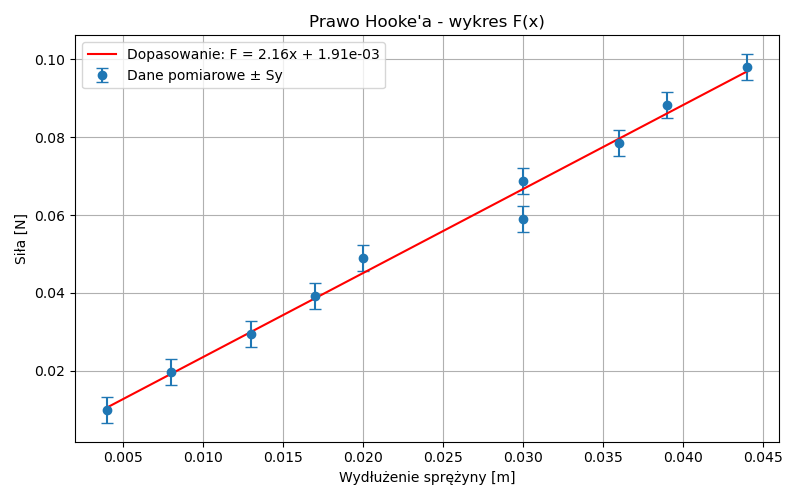
\includegraphics[width=0.9\textheight,angle=90]{Wykres_prosta_regresji_cw30.png}
    \caption{Wydłużenie sprężyny w zależności od masy obciążającej (źródło: opracowanie własne).}
    \label{fig:wykres}
\end{figure}


\bibliographystyle{plain}
\bibliography{bibliography}

\end{document}
